\documentclass[fleqn]{article}

\setlength{\oddsidemargin}{0in}
\setlength{\evensidemargin}{0in}
\setlength{\topmargin}{0.0in}
\setlength{\headheight}{0in}
\setlength{\headsep}{0in}
\setlength{\textwidth}{6.5in}
\setlength{\textheight}{9.0in}
\setlength{\parindent}{0in}
\setlength{\parskip}{0.1in}

\usepackage{amsfonts}
\usepackage{amsmath}
\usepackage{graphicx}

%opening
\begin{document}

\title{Final Project}
\author{Allen Chin, Cuauhtemoctzin Rodriguez, Brandon Tong}

\maketitle

\section*{Problem A}

	\paragraph{(a)}
		To find the approximate confidence interval for the population mean rating by men we must first find the average rating for each user, $A_i$, since ratings by the same user are not independent.
		To find $A_i$ we use the  function \texttt{tapply} to apply the \texttt{mean} function to all ratings by UserId.
		\begin{verbatim}A = tapply(rating, UserId, mean, simplify = TRUE)\end{verbatim}

		Then we need to find the mean ratings among the men. The following code snippet filters out the male users from the entire A vector and places them in mm.
		\begin{verbatim}user = read.table("./ml-100k/u.user",header = FALSE, sep ="|",quote="", 
		 col.names = c("UserId", "age", "gender", "occupation", "zipcode"))
		userGenderm = which(user$gender == 'M') #indices of the men
		mm = A[userGenderm]\end{verbatim}

		Then to find the confidence interval, we use the \texttt{t.test} function. This function calculates and displays the mean, approximate confidence interval, p-value, and other information assuming that the input data follows the student-t distruibution. Note that the student-t distribution is approximately normal for large n.
		\begin{verbatim}
			> t.test(mm)

				One Sample t-test

			data:  mm
			t = 215.9821, df = 669, p-value < 2.2e-16
			alternative hypothesis: true mean is not equal to 0
			95 percent confidence interval:
			 3.555979 3.621228
			sample estimates:
			mean of x 
			 3.588604 
		\end{verbatim}
		From the output, the approximate 95\% confidence interval for men is the interval (3.555979, 3.621228). This means that there is a 95\% chance that the mean lies within this interval. This result means that the average male user in the population will have an average of 3.58. The mean can vary 0.032624 in the interval. So there is a large proportion of 3 and 4 ratings.

	\paragraph{(b)}
		To find the approximate confidence interval for the population mean rating by women we follow the same procedure as that of men. First we find $A_i$, which yields the same result.

		Then we find the mean ratings among the women in the same way
		\begin{verbatim}user = read.table("./ml-100k/u.user",header = FALSE, sep ="|",quote="", 
		  col.names = c("UserId", "age", "gender", "occupation", "zipcode"))
		userGenderf = which(user$gender == 'F')
		mf = A[userGenderf]	#mean ratings among women\end{verbatim}

		Then to find the confidence interval, we use the \texttt{t.test} function just as before.
		\begin{verbatim}
			> t.test(mf)

				One Sample t-test

			data:  mf
			t = 123.1607, df = 272, p-value < 2.2e-16
			alternative hypothesis: true mean is not equal to 0
			95 percent confidence interval:
			 3.529837 3.644520
			sample estimates:
			mean of x 
			 3.587179 
		\end{verbatim}
		Thus, the approximate 95\% confidence interval for women is the interval (3.529837, 3.644520). The mean is slightly higher than that of the men. However this difference is insignificant because the percent difference is less than 0.04\%. We can conclude that ratings are independent of gender.

	\paragraph{(c)}
		To find an approximate 95\% confidence interval for the difference between the two means we use equations (10.21) and (9.23) from the text.
		Let \((\overline{M}, s_m^2, n_m)\) and \((\overline{F}, s_f^2, n_f)\) denote the sample mean, sample variance, and sample size for ratings among males and females. Applying equation (10.18) with the same assumptions as in section 10.6, the standard error for the difference of two sample means is 
		\[s.e.(\overline{M} - \overline{F}) = \sqrt{\frac{s_m^2}{n_m} + \frac{s_f^2}{n_f}} \tag{10.18}\]
		The above formula applies when the two estimators are independent. We assume that they are, as there is no foreseeable reason why the ratings of male critics should impact ratings of female critics. We apply the standard error to equation (10.21).

		Using mm and mf from parts a and b, we use the following code: 
		\begin{verbatim}
			Mbar = 3.588604	#from t.test results
			Fbar = 3.587179

			#find s by eqn 9.23
			Nmen = length(mm)
			Nwomen = length(mf)
			s2men = 1/Nmen*sum((mm - Mbar)^2)
			s2women = 1/Nwomen*sum((mf - Fbar)^2)

			# find interval with eqn 10.21
			marginOfError = 1.96*sqrt(s2men/Nmen + s2women/Nwomen)
			
			interval = c(Mbar - Fbar - marginOfError, Mbar - Fbar + marginOfError)
		\end{verbatim}
		Thus, the approximate 95\% confidence interval for the difference between the mean men ratings and mean women ratings is the interval (-0.06419468,  0.06704468). This is another way of showing that the rating is independent of gender.
	
	\paragraph{(d)}
		We wish to test the significance of the difference between two means, in other words the null hypothesis \(H_0 : \theta = c\). To do so we need to find  
		\[Z = \frac{\hat{\theta} - c}{s.e.(\hat{\theta})} \tag{11.6}\]
		
		Using the same assumptions as part c,
		
		
		Noting that for the hypothesis, \(\theta = \overline{M} - \overline{F}\) and \(c = 0\), 
		\begin{align*}
		Z &= \frac{\hat{\theta} - c}{s.e.(\hat{\theta})}\\
		  &= \frac{\overline{M} - \overline{F}}{s.e.(\overline{M} - \overline{F})}\\
		  &= \frac{3.588604 - 3.587179}{0.03347943}\\
		  &= 0.04256345
		\end{align*}
		Since \(|Z| < 1.96\), we accept the null hypothesis at the significance level of \(\alpha = 0.05\). This signifance test signifies that the difference between the mean for women and men is very close to 0. In other words, the difference is close enough to consider it to be 0.

	\paragraph{(e)}
		The following figure is a histogram of male and female ratings displayed on the same graph. This shows that the bulk of ratings for both genders are 3's and 4's.\\
		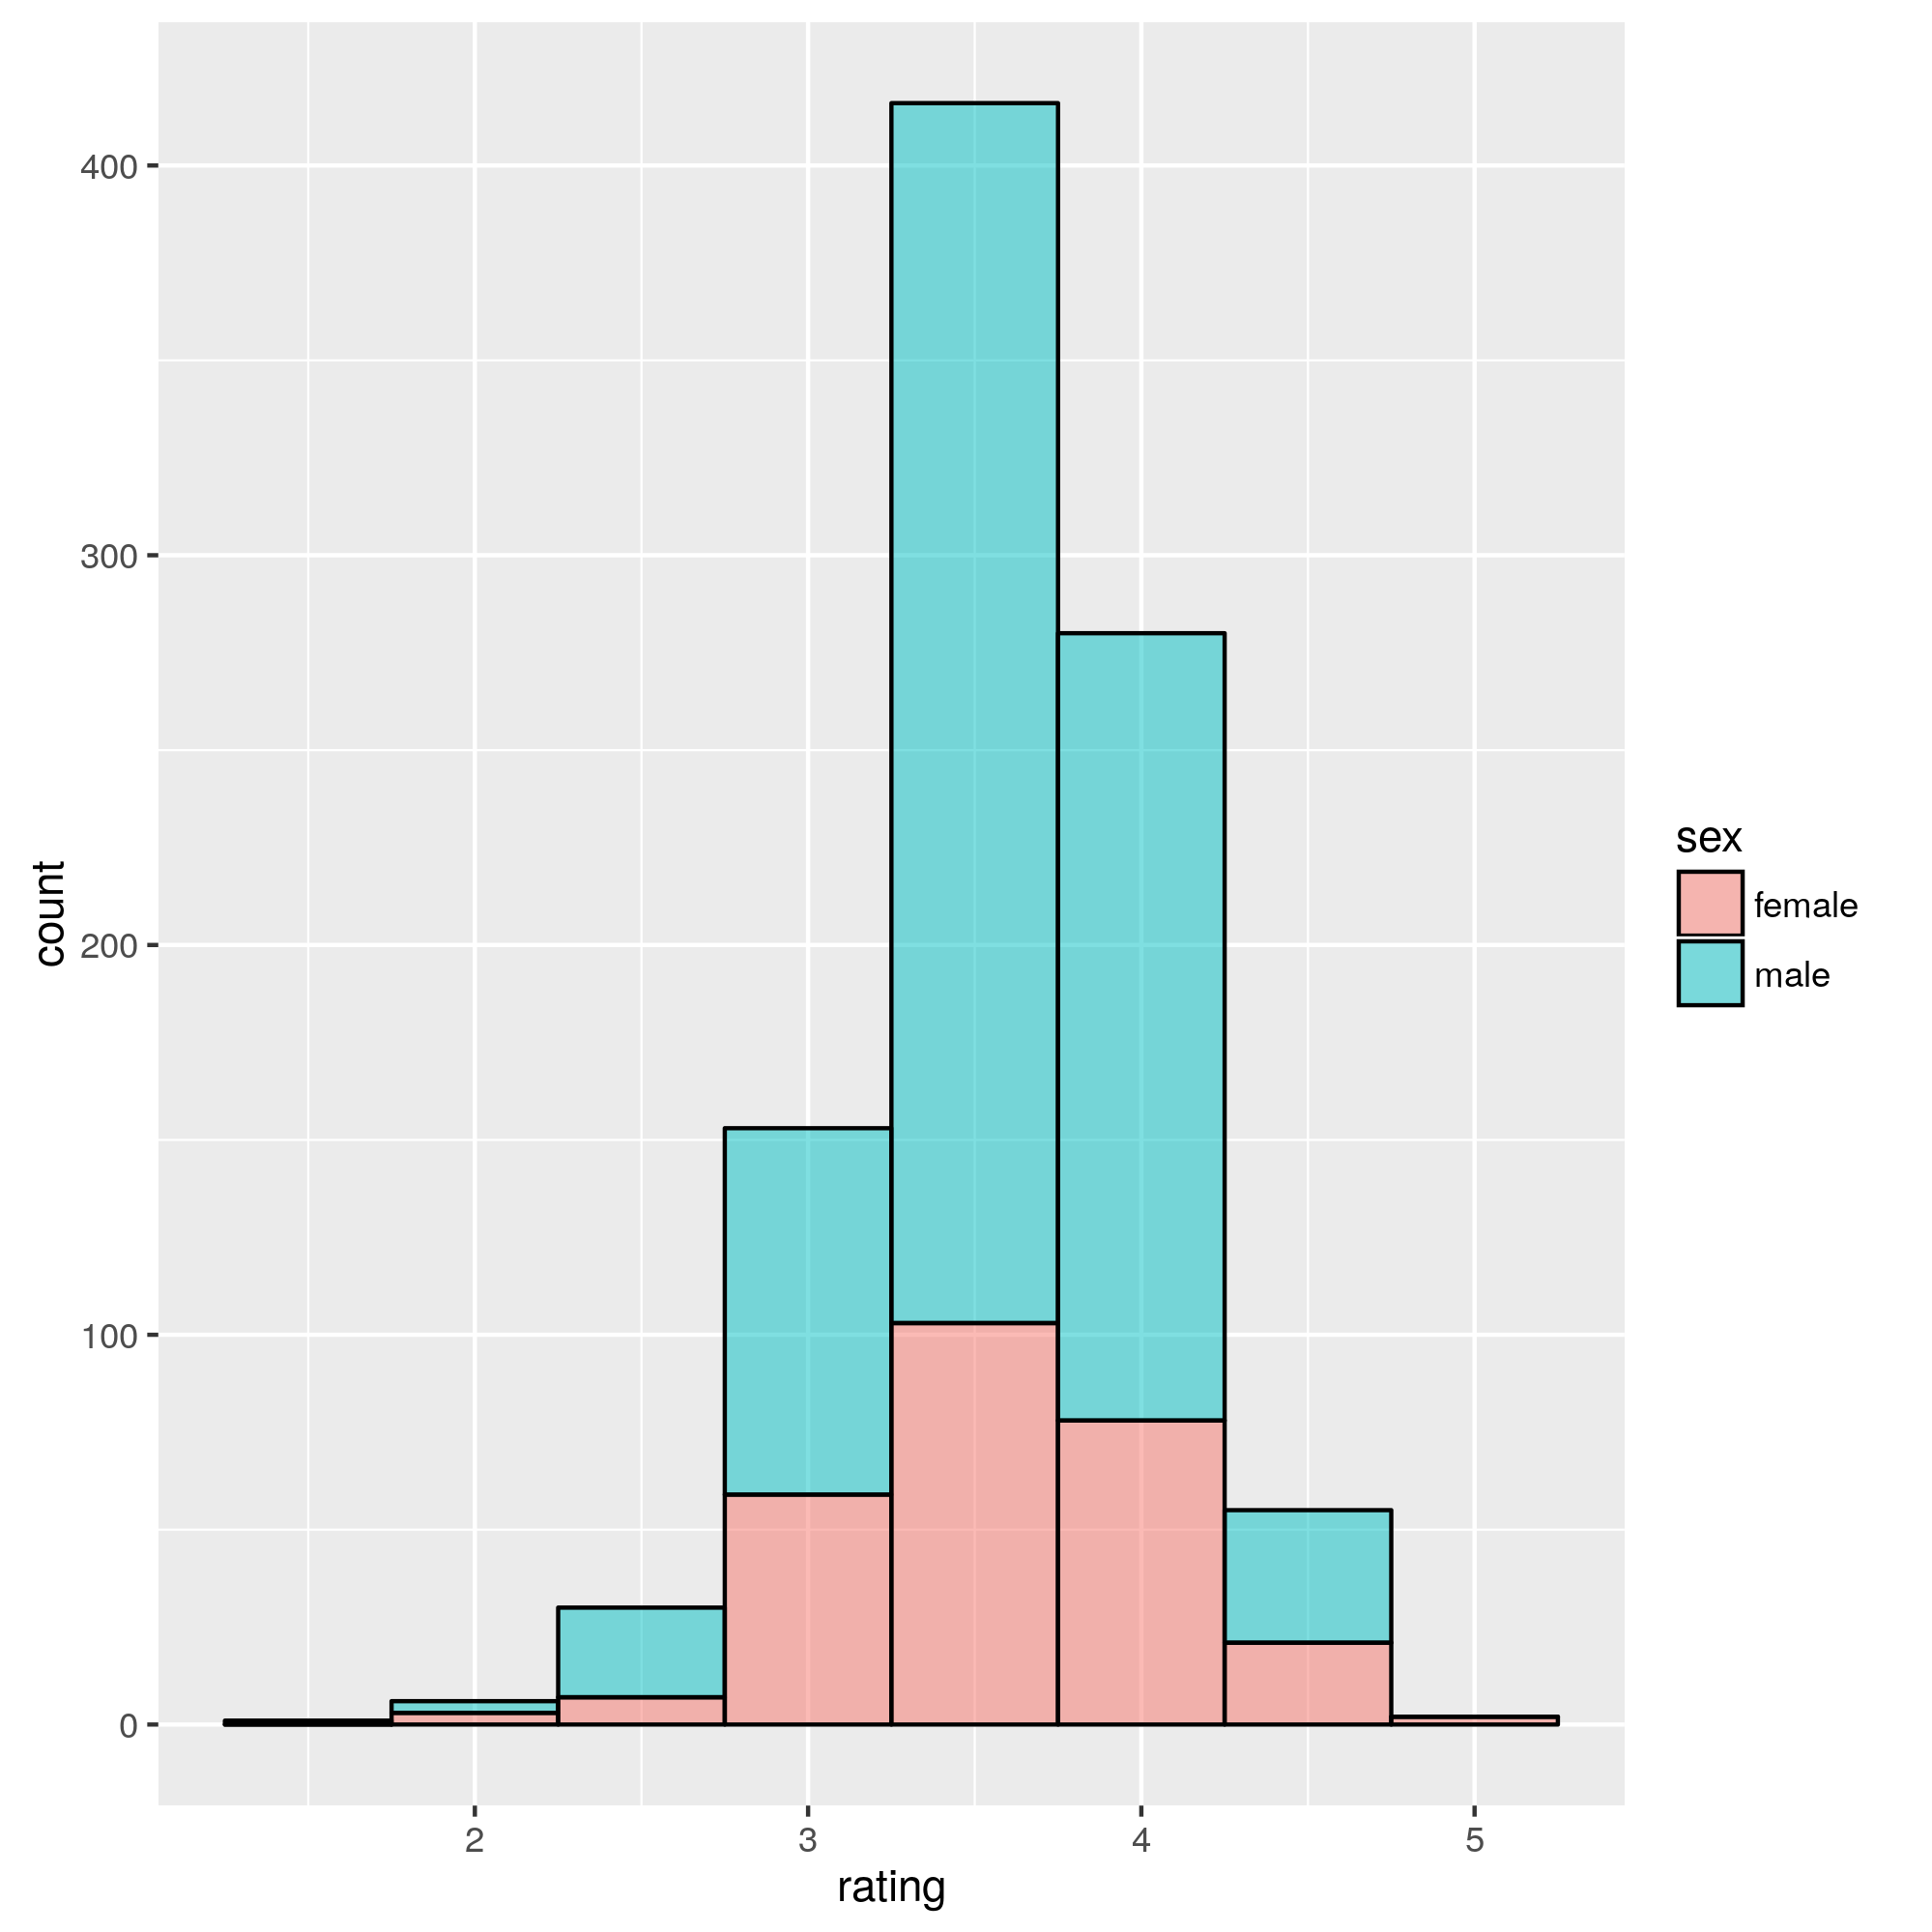
\includegraphics{plot.png} 

	 
	\paragraph{(f)}
		We are asked to find an approximate 95\% confidence interval for the difference between the population mean number of ratings by men and women. To do so we first find the number of ratings of each user. Define this quantity $B$, named \texttt{NumRat} in the code.

		We find this value in the same way we find $A$ but use length instead of mean since we are interested in the number of ratings not the mean of the ratings

		\begin{verbatim}NumRat = tapply(rating, UserId, length, simplify = TRUE)\end{verbatim}

		Then we assume that the ratings make a random sample as defined in section 9.1.1 in the text.
		This implies that the population mean can be approximated with the sample mean as described in 9.2.4.

		So using \texttt{t.test()} and the same method as in part c we yield the interval (2.504417, 30.595763). The \texttt{t.test()} results and the interval show that there is a difference between the mean number of ratings for men and women but since this interval is so large, we cannot confidently make a conclusion about the difference between the number of ratings of men and women. All we can conclude is that this difference is between (2.504417, 30.595763) with 95\% chance. Since the difference is positive, we can conclude that men have a larger mean number of ratings.


	\paragraph{(g)}
		We want to find the approxiamte 95\% confidence interval for the population proportion of users who are men. To do this, we first calculate $ \hat{p}$. $\hat{p}$ is equivalent to the number of male users divided by the total number of male and female users. 

		Using the values from part a, and using the \texttt{unique()} function, we can remove all duplicate UserIds.
		\begin{verbatim}allUnique = unique(allRed, by = UserId)\end{verbatim}

		Then with \begin{verbatim}numM = sum(allUnique == 'M')\end{verbatim} we determine the total number of male users. We replace 'M' with 'F' for female users. With simple math, we can determine $\hat{p}$.

		Now we find the margin of error, which is 1.96 multiplied by the standard deviation divided by the sqaure root of the total number of men. Alternatively, we can find the numeber of male useres by using \texttt{mm} from the previous problems 
		\begin{verbatim}Nmen = length(mm)\end{verbatim} 
		This determines the number of male users. After, we borrow \texttt{Mbar} from the t.test results to calculate the standard deviation.
		\begin{verbatim}smen = sqrt(1/Nmen*sum((mm-Mbar)^2))\end{verbatim}
		Margin of Error:\begin{verbatim} marginOfError = 1.96*smen/sqrt(nmen)\end{verbatim}
		Lastly, we construct our interval which is defined to be \begin{verbatim} interval = c(phat - marginOfError, phat + marginOfError)\end{verbatim}
		
		Our interval is: (0.6779568, 0.7430401)

		This means that there is a larger proportion of males than females. This makes sense since there are more male users in the user file given in the data set.

	\paragraph{(h.1)}
		We are asked to form a confidence interval for $\beta_{age}$, and test the hypothesis that that coefficient is 0. Where, $\beta_{age}$ is the coefficient for the age varaible in the linear regression equation. To do so we use the \texttt{lm()} and \texttt{summary()} functions as done in section 12.6 of the text. Where we form a linear model of rating in terms of age and gender. We therefore run the following code:
		\begin{verbatim} 
			> all = read.table("u.all",header = TRUE, sep ="|",quote="")
			> summary(lm(formula = all$rating ~ all$age + all$gender))

			Call:
			lm(formula = all$rating ~ all$age + all$gender)

			Residuals:
			    Min      1Q  Median      3Q     Max 
			-2.7407 -0.5617  0.3921  0.5355  1.6098 

			Coefficients:
			              Estimate Std. Error t value Pr(>|t|)    
			(Intercept)  3.3598944  0.0121603 276.299   <2e-16 ***
			all$age      0.0053107  0.0003076  17.266   <2e-16 ***
			all$genderM -0.0069035  0.0081345  -0.849    0.396    
			---
			Signif. codes:  0 ‘***’ 0.001 ‘**’ 0.01 ‘*’ 0.05 ‘.’ 0.1 ‘ ’ 1

			Residual standard error: 1.124 on 99997 degrees of freedom
			Multiple R-squared:  0.002973,	Adjusted R-squared:  0.002953 
			F-statistic: 149.1 on 2 and 99997 DF,  p-value: < 2.2e-16
		\end{verbatim}
		We then form the confidence interval through equation 10.15 and the standard error.
		\begin{verbatim} 
			> BetaAge = 0.0053107
			> stdError = 0.0003076
			> interval = c(BetaAge - 1.96*stdError, BetaAge + 1.96*stdError)
			> interval
			[1] 0.004707804 0.005913596
		\end{verbatim} 

		Thus our 95\% confidence interval is (0.004707804, 0.005913596)
		To perform our significance test of $H_0: \beta_{age} =0$ we calculate
		$Z = \frac{\beta_{age} - 0}{se(\beta_{age})} = \frac{0.0053107 - 0}{0.0003076}$
		or we can look at the t value column in the results to find 17.266.

		Since 17.266 is much larger than 1.96 we can reject the null hypothesis.

	\paragraph{(h.2)}
		To form a confidence interval for the mean population rating among women of age 28 we follow the methods in section 12.11.
		Note that the levels for women and men are 1 and 2, respectively. So we use \texttt{vcov()} to find the matrix A, and use the previous results for $\beta$.
		Note we use the vector t = (1, 28, 1) to represent women of age 28. Where, the 1st 1 represents setting the first $t$ coefficient to 1, 28 represents users of age 28, and the 2nd 1 represents females.

		We use the code:
		\begin{verbatim}
		all = read.table("u.all",header = TRUE, sep ="|",quote="")

		#following section 12.11
		lmout = lm(formula = all$rating ~ all$age + all$gender)
		A = vcov(lmout)
		#levels(all$gender) 	#female = 1
		#[1] "F" "M"
		b = matrix(c(1,28,1), ncol = 3)
		varHat = b %*% A %*% t(b)

		stdError = sqrt(varHat)
		stdError = stdError[1,1]

		beta = c(3.3598944, 0.0053107, -0.0069035)
		meanRatWomen28 = sum(c(1, 28, 1)*beta)

		interval = c(meanRatWomen28 - 1.96*stdError, meanRatWomen28 + 1.96*stdError)
		\end{verbatim}
		We yield the interval (3.493020, 3.510361)
		This means that the average 28 year old women had an average rating between 3.493020 and 3.510361 with a 95\% chance. This shows that 28 year old women rate slightly lower than the average woman.
		

\section*{Problem B}

	We are asked to predict vocabulary size from age (in months), birth order, ethnicity, sex and mom's education, using a linear regression model. Natuarlly, we aim to use R's \texttt{lm()} function.
	We start by loading the raw data into a data frame called \texttt{vocab}.

	\begin{verbatim}vocab = read.table("./wordbank/vocabulary_norms_data.csv",header = TRUE, sep =",",quote="")\end{verbatim}

	Then we designed indicator variables for each "group". We have indicator variables for each birth order, ethnicity, and education. We chose to perform linear model analysis on each "group" individually because including all the indicator variables would increase the chances of overfitting the model and resulting in less helpful results. 

	We split each "group" into its own function. Starting with birth order, we made an indicator variable for each birth order 1 through 8. We then used \texttt{lm()} to predict vacabulary size based on birth order.

	\begin{verbatim}lmout = summary(lm(vocab$X.vocab ~ b1 + b2 + b3 + b4 + b5 + b6 + b7 + b8))\end{verbatim}

	We encountered a problem. The birth order for 8 shows NA at the results

	\begin{verbatim}
		Coefficients: (1 not defined because of singularities)
		            Estimate Std. Error t value Pr(>|t|)
		(Intercept)      4.0      203.2   0.020    0.984
		b1             292.4      203.3   1.438    0.150
		b2             260.0      203.3   1.279    0.201
		b3             218.5      203.6   1.073    0.283
		b4             248.7      204.3   1.217    0.224
		b5             198.9      208.2   0.955    0.339
		b6             195.4      213.1   0.917    0.359
		b7              59.5      227.2   0.262    0.793
		b8                NA         NA      NA       NA
	\end{verbatim}

	This is explained in section 12.15.3 of the text book. The problem is that since they are all indicator variables, one of the equations is redundant. In other words b8 is linearly dependent on the other equations. Since this means the inverse cannot be found, \texttt{lm()} ommited it and called it a "singularity".
	Ignoring b8 we can see a decrease in vocabulary as birth order increases. To consolidate b8 we run \texttt{lm()} again but this time we manually omit b1 so that b8 is included. This works but we recieve different coefficients. However we can see that b8 still follows the same trend of decreasing vocabulary with higher birth order. As a result we cannot find the exact coefficent of each b value, but we can verify the decreasing trend for every single one.

	Also note that the standard error increases as birth order increases. This is due there being less data on the higher birth oders since one is less likely to have more kids than less.
	The following is a graphical representation of the previous coefficients.\\

	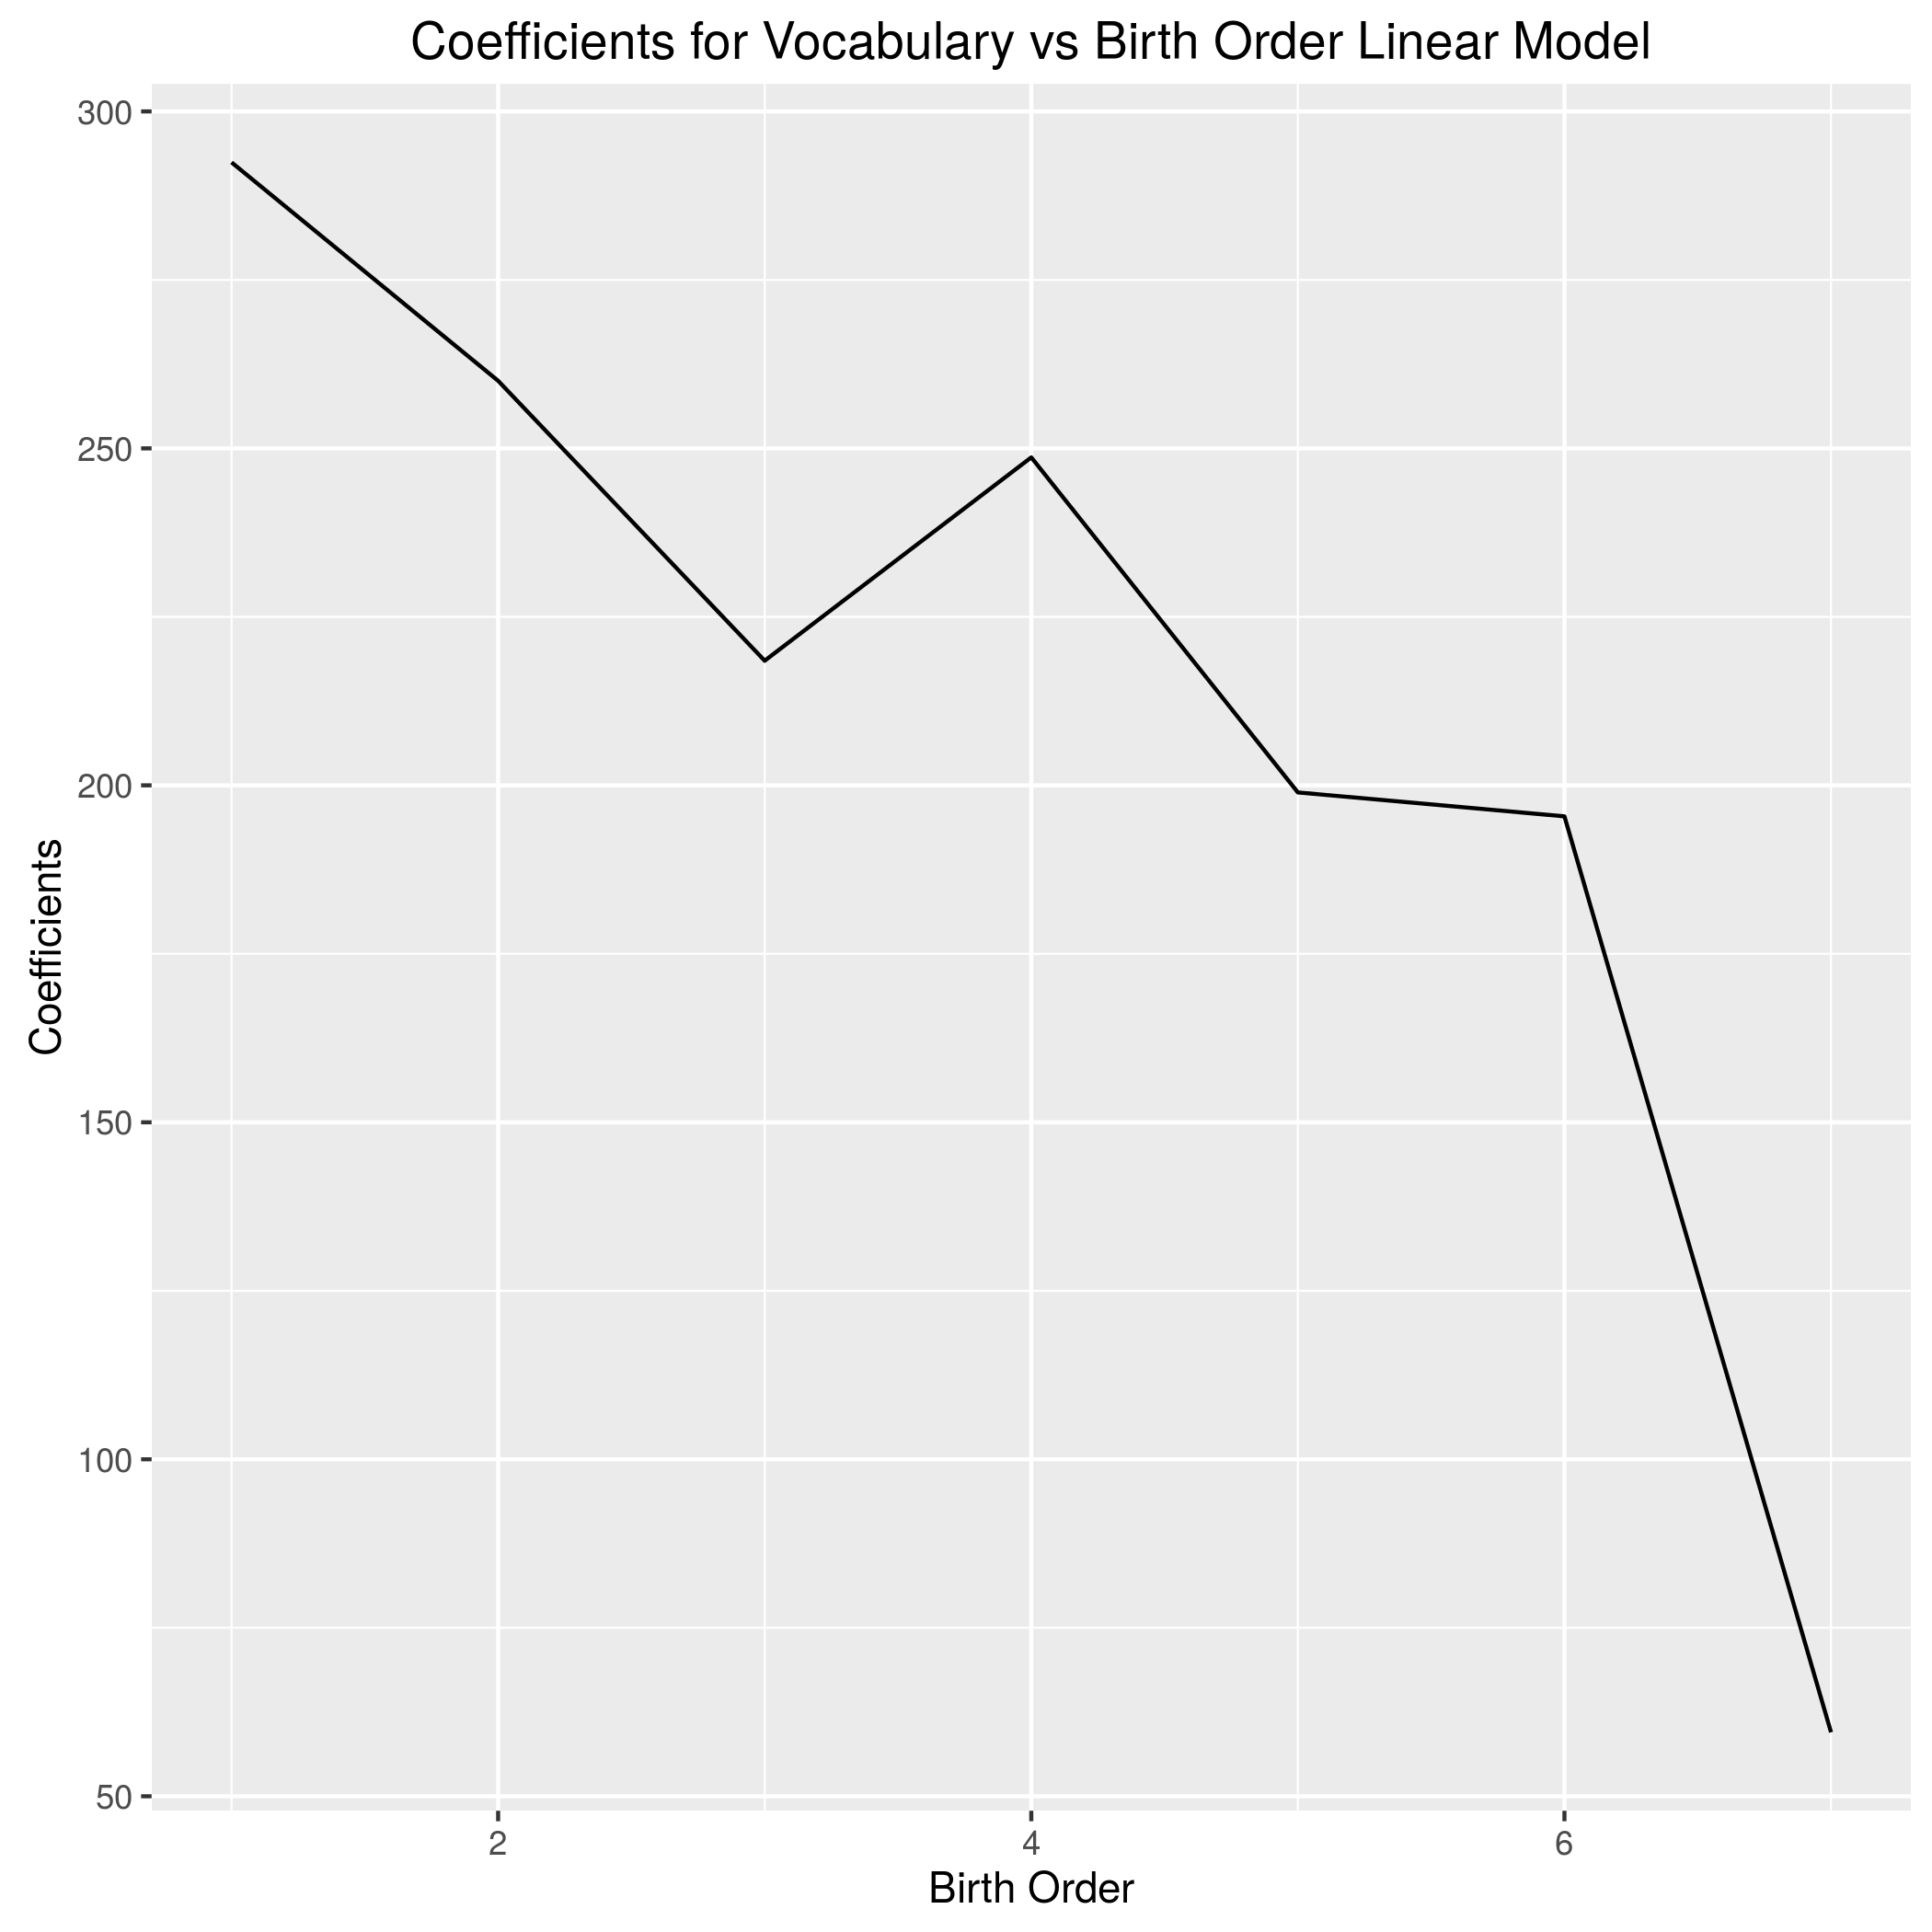
\includegraphics{BirthOrder.png}

	We perform a simpler linear model analysis with the age variable. This is predicting vacobulary size soley on age in months. We run
	\begin{verbatim}summary(lm(vocab$X.vocab ~ vocab$X.age.))\end{verbatim}
	And our results are:
	\begin{verbatim}
	Coefficients:
              	      Estimate Std. Error t value Pr(>|t|)
	(Intercept)  -503.3810     9.2151  -54.63   <2e-16 ***
	vocab$X.age.   34.4475     0.4037   85.32   <2e-16 ***
	\end{verbatim}
	These results mean that according to the standard error, we can confidently say that increasing age by one month results in 34.4 more words learned. This result makes intuitive sense since a toddler learns more words as they age.

	We perform a linear model analysis similar to that for birth order for the mother's education level. We also encounter the same multicollinearity as before since we are using indicator variables again.

	We ran \texttt{lm()} with the education levels in order of degree level to easily find trends.
	\begin{verbatim}summary(lm(vocab$X.vocab ~ prim + someSec +sec +   someCollege  +college + someGrad + grad ))\end{verbatim}
	We had to run \texttt{lm()} twice for the same reason discussed above.

	We yield the following:
	\begin{verbatim}
	Coefficients: (1 not defined because of singularities)
	             Estimate Std. Error t value Pr(>|t|)    
	(Intercept)  289.1352     8.5078  33.985  < 2e-16 ***
	prim        -144.6352    72.7530  -1.988 0.046907 *  
	someSec      -66.0883    19.9668  -3.310 0.000945 ***
	sec           -2.9366    12.9938  -0.226 0.821219    
	someCollege  -26.6593    11.9111  -2.238 0.025289 *  
	college      -12.6599    11.0235  -1.148 0.250886    
	someGrad       0.4126    18.3957   0.022 0.982108    
	grad               NA         NA      NA       NA
	\end{verbatim}
	One can see that the coefficients increase as education level increases. Some College and College don't exactly fit the trend but we must keep in mind that the standard errors are quite large and we can see that there is overlap in the possible values for each coefficient. In addition we can also see that there is a general trend from the graphial representation.\\
	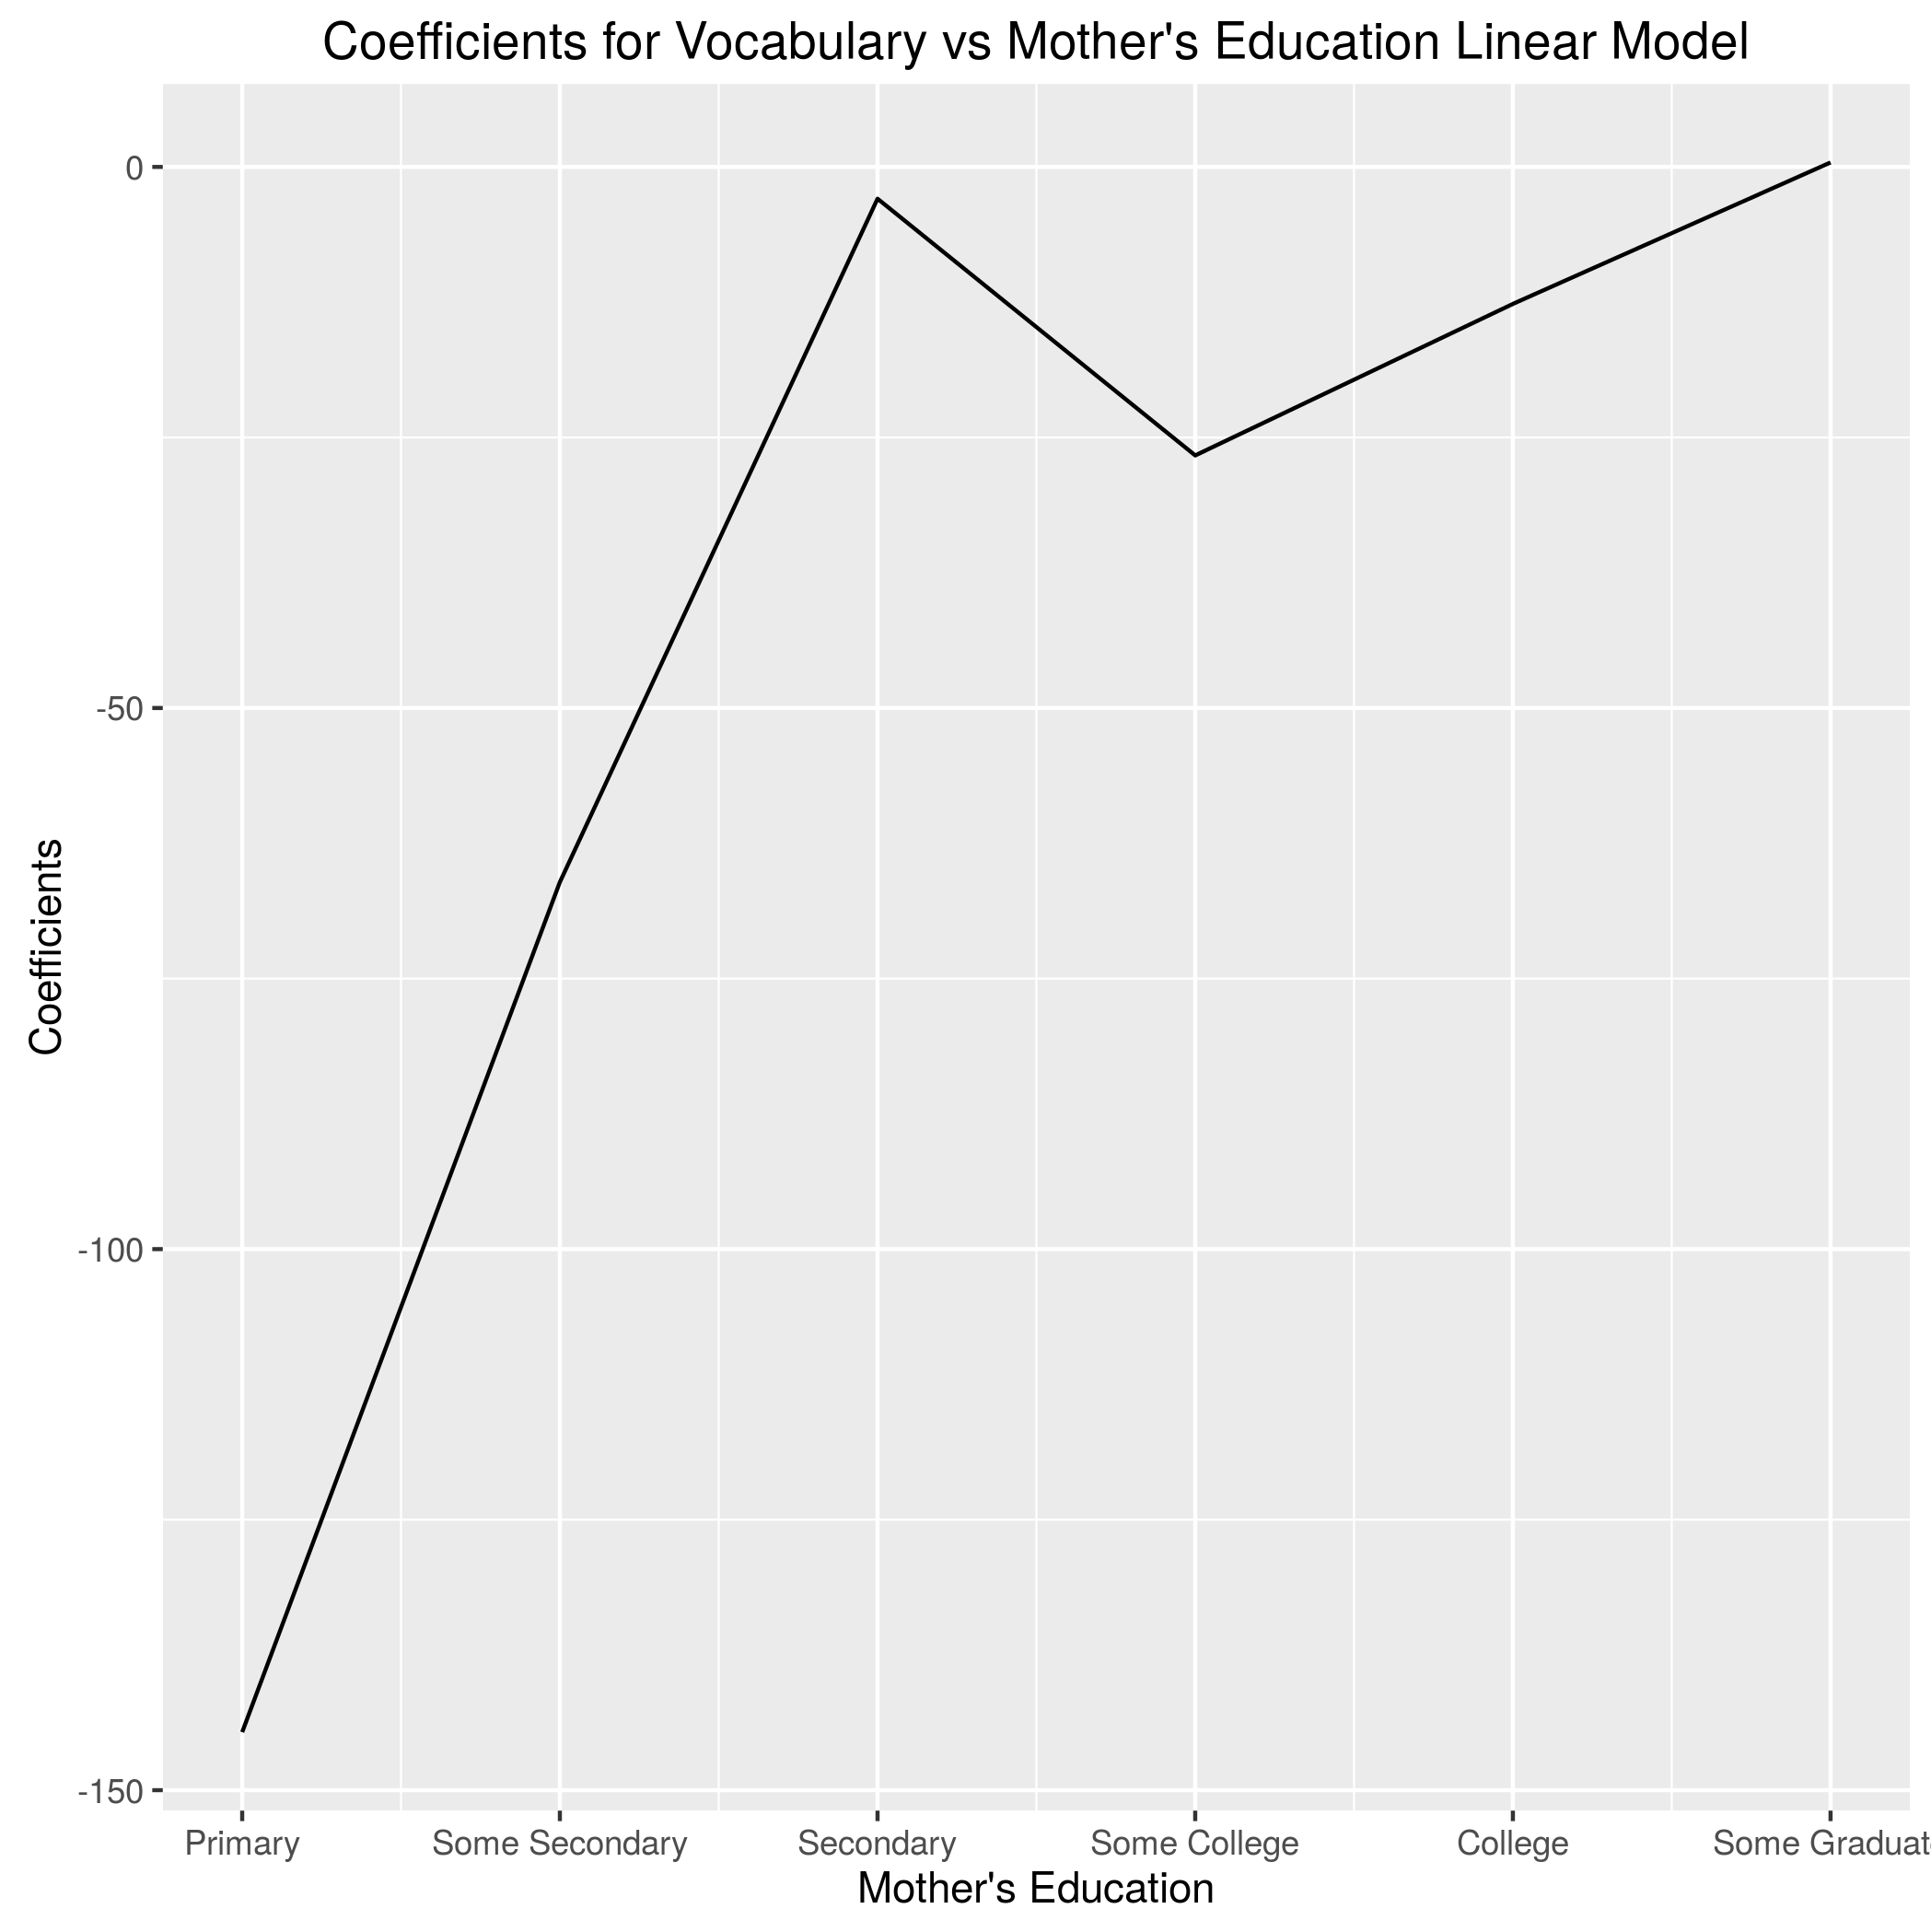
\includegraphics{MomEd.png}

	We used the same methods to analyze ethnicity. We run \texttt{lm()} twice again and yield the following:

	\begin{verbatim}
		Coefficients: (1 not defined because of singularities)
		            Estimate Std. Error t value Pr(>|t|)    
		(Intercept)  280.320      4.327  64.783  < 2e-16 ***
		asian        -16.376     24.622  -0.665  0.50605    
		black          3.429     14.118   0.243  0.80809    
		hisp         -57.071     18.231  -3.130  0.00176 ** 
		other        -54.900     20.878  -2.630  0.00860 ** 
		white             NA         NA      NA       NA    
		---

		Call:
		lm(formula = vocab$X.vocab ~ white + asian + black + hisp + other)

		Residuals:
		    Min      1Q  Median      3Q     Max 
		-280.32 -191.63  -33.32  178.68  446.58 

		Coefficients: (1 not defined because of singularities)
		            Estimate Std. Error t value Pr(>|t|)    
		(Intercept)  225.420     20.424  11.037   <2e-16 ***
		white         54.900     20.878   2.630   0.0086 ** 
		asian         38.524     31.697   1.215   0.2243    
		black         58.329     24.449   2.386   0.0171 *  
		hisp          -2.172     27.033  -0.080   0.9360    
		other             NA         NA      NA       NA
	\end{verbatim}
	One can see that there is no general trend in this result. This can be seen in two ways. 1) There is not a significant increase or decrease between coefficients. 2) The standard errors are so large that the slight coefficient differences are not significant since each ethnicity has large overlap with every other ethnicity. Therefore, we can conclude that vocabulary size has no dependence on ethnicity. This make sense since there is no reason that different ethnicities should perform differently.

	And finally, gender. We used indicator variables and resorted to the same solution. We call \texttt{lm()} just like we have before.
	\begin{verbatim}summary(lm(vocab$X.vocab ~ f + m))\end{verbatim}
	And we yield the results
	\begin{verbatim}
		Coefficients: (1 not defined because of singularities)
		            Estimate Std. Error t value Pr(>|t|)    
		(Intercept)  259.285      4.793  54.096  < 2e-16 ***
		f             36.789      6.872   5.354  9.1e-08 ***
		m                 NA         NA      NA       NA    
		---

		Call:
		lm(formula = vocab$X.vocab ~ m + f)

		Residuals:
		    Min      1Q  Median      3Q     Max 
		-295.07 -213.29  -41.07  202.77  420.71 

		Coefficients: (1 not defined because of singularities)
		            Estimate Std. Error t value Pr(>|t|)    
		(Intercept)  296.074      4.924  60.124  < 2e-16 ***
		m            -36.789      6.872  -5.354  9.1e-08 ***
		f                 NA         NA      NA       NA 
	\end{verbatim}
	One can see from these results that females have a better vocabulary. Being a female at any age puts one at a 37 word advantage over the male counter parts. This is an interesting result. It is known that females mature quicker than males but we can also see this matches our results.

	Despite our data showing linear trends, we must remember that our sample population may have large standard errors that skew the accuracy of our results. For example, the birth order data set had very larger errors due to higher birth orders having less members. So the data showing a higher birth order leading to a smaller vocabulary is less accurate. On the other hand, our male or female data set had small errors, making it safer to say females learn sligtly more vocabulary words than males. The larger the error, the harder it is to draw relationships between our data sets. 

\appendix

Brandon Tong: Wrote function and the write up for 1g), also rechecked all other parts of problem 1. Everyone collaboratively worked on the functions for problem2. 
	
\end{document}
